\documentclass[a4paper,12pt]{article}
\usepackage[latin1]{inputenc}
\usepackage[pdftex]{color,graphicx}
\usepackage[hypertexnames=false]{hyperref} 
\usepackage[german,ngerman]{babel}
\usepackage{fancyhdr}
\usepackage{amssymb}
\usepackage{background}
\usepackage{amsmath}
\usepackage[rflt]{floatflt}
\usepackage{tabularx}
\usepackage{ausarbeitung}
\usepackage{listings}
\usepackage{color}

\definecolor{mygreen}{rgb}{0,0.6,0}
\definecolor{mygray}{rgb}{0.5,0.5,0.5}

\lstset{basicstyle=\scriptsize, numbers=left, numberstyle=\tiny\color{mygray}, numbersep=5pt, basicstyle=\footnotesize\ttfamily,
  keywordstyle=\bfseries\color{green!40!black},
  commentstyle=\itshape\color{purple!40!black},
  stringstyle=\color{orange},breaklines=true}

%% Diese Farben werden f�r den Quelltext verwendet
\definecolor{srcblue}{rgb}{0,0,0.5}
\definecolor{srcgray}{rgb}{0.5,0.5,0.5}
\definecolor{srcred}{rgb}{0.5,0,0}

\renewcommand{\lstlistingname}{Quellcode}% Listing -> Algorithm
\renewcommand{\lstlistlistingname}{\lstlistingname verzeichnis}% List of Listings

%% Diese Zeile unbedingt stehen lassen und anpassen - sie enth�lt Autor und Titel der Ausarbeitung
\mywork{David Bujok}{Thema der Arbeit}

\begin{document}
\SetBgContents{}
	%% Bei Diplomarbeiten folgende Zeile nutzen
	\mybachelortitle{Dipl.-Wirt.Inform. Claus Alexander Usener}
	%% Bei Bachelorarbeiten diese Zeile auskommentieren
	%%\mybachelortitle{(ggf. Name des Betreuers)}
	%% Bei Seminararbeiten diese Zeile auskommentieren
	%%\myseminartitle{Titel des Seminars}{(ggf. Name des Betreuers)}

  %% Inhaltsverzeichnis
  %% frontmatter setzt die Seitenzahlen auf i, ii, ...
  \frontmatter

	%% Generiert automatisch aus den Sektionsbefehlen ein Inhaltsverzeichnis  
  \tableofcontents
  \newpage
	\lstlistoflistings
	\newpage
	\listoffigures
  \newpage

	%% das Mainmatter sorgt f�r die Nutzung arabischer Seitenzahlen
	\mainmatter
	
\section{Einleitung}
\label{sec:einleitung}

Bei Moodle handelt es sich um ein Softwarepaket, welches einen  konstruktivistischen Lehr- und Lernansatz unterst�tzt. \cite{moo15a}
 Weltweit in 231 L�ndern �ber 53.000 Seiten registriert \cite{moo15a}
 
 Moodle ist international die am weitesten verbreitete Lernplattform \cite{hei15}.
 
%Moodle ist eine frei verf�gbare Open Source Software. Dies bedeutet, dass sie frei erhaeltlich ist. Au�erdem bietet Sie die M�glichkeit der individuellen Anpassung an spezifische Anwendungssituationen \cite{moo15a}.

Die Westf�lische Wilhelms-Universit�t M�nster stellt zur Verbesserung des Lehrbetriebs eine Moodledistribution unter dem Namen Learnweb zur Verf�gung.

F�r die Vorlesung \textit{Informatik I} wurde bereits ein Moodlemodul implementiert, welches die M�glichkeit  bietet ????

Die Arbeit wird durch ein Grundlagenkapitel (Kapitel \ref{sec:grundlagen}) eingeleitet, in die zentralen Ideen von E-Assessment vorgestellt und 
die wesentlichen Merkmale der Lernplattform Moodle hervorgehoben werden. Bei der Vorstellung von Moodle wird auf die Pluginstruktur der Plattform eingegangen. 

Im darauffolgenden Kapitel (Kapitel \ref{sec:dsbuilder}) wird das Modul EASy-DSBuilder vorgestellt. Hierbei wird auf die Funktionalit�t aus Benutzersicht und auf die Struktur aus technischer Sicht eingegangen.


\subsubsection{Aufbau eines Plugins}
\label{sec:aufbauPlugin}

F�r jedes Plugin in Moodle muss eine bestimmte Datenstruktur implementiert werden. Diese besteht aus separaten Unterverzeichnissen und verpflichtenden Dateien. Des weiteren haben Entwickler die M�glichkeit weitere Dateien selbst zu gestalten. 

\paragraph{/backup}

\paragraph{/db}
\begin{itemize} 
	\item \textbf{/access.php}
	\item \textbf{/install.xml}
	\item \textbf{log.php}
	\item \textbf{upgrade.php}
\end{itemize}
\paragraph{/lang}

\paragraph{/}
\section{Vorstellung des Moodlemoduls EASy-DSBuilder}
\label{sec:dsbuilder}
Der EASy-DSBuilder ist ein E-Assessent Tool, welches der Evaluation grundlegender Konzepte �ber Operationen (z.B. Suchen, Einf�gen, und Entfernen) innerhalb der Datenstruktur \textit{Bin�rbaum} dient \cite{Usener2014}.
Das Tool wurde speziell f�r die Lernplattform Moodle implementiert. 

Diese Kapitel wird das Tool EASy-DSBuilder vorstellen. Hierbei wird zu erst in Kapitel \ref{sec:funktionalitaet} auf die Funktionalit�t aus Benutzersicht eingegangen. Anschlie�end erfolgt eine Erl�uterung der technischen Umsetzung (Kapitel \ref{sec:technologien}).

\subsection{Funktionalit�t aus Benutzersicht}
\label{sec:funktionalitaet}

Im folgenden Kapitel wird die Funktionalit�t des Moodlemodul EASy-DSBuilder vorgestellt. Hierbei wird auf die beiden Sichten Studierender und Lehrender eingegangen.

\paragraph{Lehrender} \hfill \\
Der Lehrende hat zwei grundlegende Aufgaben. Zum Einen ist er daf�r verantwortlich, dass eine Aufgabe erstellt wird, zum Anderen hat er die M�glichkeit, die Abgaben einzusehen, um sie beispielsweise zu bewerten oder Indikatoren zur Verbesserung der Lehre zu finden \cite{Usener2014}. Wird eine neue Aufgabe erstellt, hat der Lehrende die M�glichkeit allgemeine Informationen wie den \textit{Titel}, die \textit{Beschreibung} und das \textit{F�lligkeitsdatum} anzugeben. Unter \textit{Source Files} kann der Lehrende �ber Drag-and-Drop seine eigene Implementierung einer Datenstruktur zu dem Moodlemodul hinzuf�gen. Hierzu muss er einen Wrapper auf Basis des Interfaces \textit{DataStructureWrapperInterface<K extends Comparable<K>, D>} implementieren (vergl. Anhang, Quellcode \ref{code:wrapper}). Diese Wrapperklasse muss anschlie�end vom Lehrenden als Hauptklasse eingestellt werden. Auf die Funktionalit�t der Wrapperklasse aus technischer Sicht wird im Kapitel \ref{sec:technWebService} n�her eingegangen. Des weiteren kann der Lehrende eine Feedback aktivieren. Die genau Funktionalit�t des Feedbacks wird im Abschnitt �ber die Funktionalit�t aus Sicht des Studierenden erl�utert.  

\paragraph{Studierender} \hfill \\
Der Studierende verf�gt �ber zwei Ansichten. Zum einen gibt es die �bersichtsansicht, zum anderen die Bearbeitungsansicht.
Nachdem der Studierende sich in das Modul eingew�hlt hat, ist die �bersichtsansicht �ber den bisherigen Verlauf des Assessments zu sehen. In dieser �bersicht ist der Abgabestatus, der Bewertungsstand, der Abgabezeitpunkt und die verbliebene Zeit zu sehen (vergl. Abb. \ref{}). �ber den Button \textit{Aufgabe bearbeiten} gelangt der Studierende zum Editor, in dem die Aufgabe bearbeitet werden kann. 

Die Bearbeitungsansicht ist in drei grundlegende Abschnitte unterteilt. Den oberen Teil der Ansicht bildet ein �berblick �ber den aktuellen Schritt. Dieser �berblick beinhaltet den Fortschritt der Aufgabe, die Nummer des aktuellen Schritts und den aktuellen Arbeitsauftrag. 
\begin{figure}[htbp] 
  \centering
     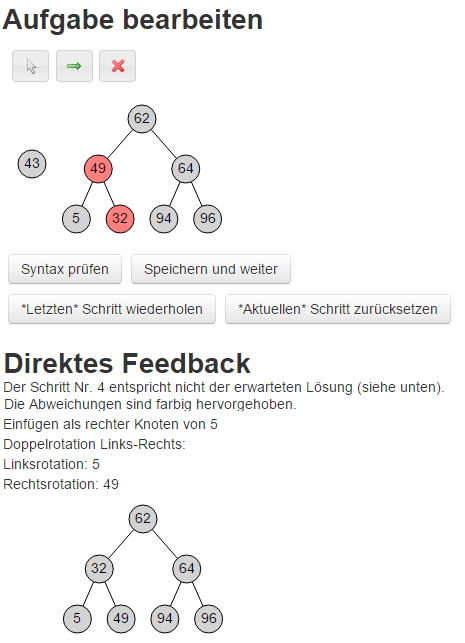
\includegraphics[width=0.5\textwidth]{graphics/editor.jpg}
  \caption{DSBuilder Editor}
  \label{fig:editor}
\end{figure}
Im mittleren Teil der Sicht befindet sich der Editor, in dem der Studierende die Aufgabe bearbeiten kann. Im oberen linken Bereich des Editor befinden sich drei Kn�pfe (vergl. Abb. \ref{fig:editor}), �ber welche der Editiermodus ausgew�hlt werden kann. Der 1. Knopf erm�glicht das verschieben von Konten im Editor, der zweite Knopf erm�glicht das Ziehen von Kanten zwischen zwei Knoten, und der dritte Knopf erm�glicht das Entfernen von Kanten.

Der Drag-and-Drop-Grafikeditor enth�lt zwei bearbeitbare Elemente, die Knoten und die Kanten. �ber Manipulation dieser Elemente sollen Studierende den
Umgang mit Datenstrukturoperationen erlernen. Hierbei k�nnte der Studierende Operationen wie das Einf�gen eines Elements in oder das L�schen eines Elements aus einer Datenstruktur 
praktizieren. In der momentanen Version des EASyDSBuilders kann der Studierende nur das Einf�gen Praktizieren. Weiterhin beginnt in dieser Version jeder Schritt mit dem Ergebnisbaum des zuvor eingereichten Schritts, oder einem Initiierngsbaum,
falls es sich um den  ersten Schritt handelt.
Auf der linken Seite des Editors wird der einzuf�gende Knoten bereitgestellt. Die Aufgabe des Studierenden ist es nun, diesen Knoten an der richtigen 
Stelle in den Baum einzuf�gen. Hierbei kann er sich dem Verschieben der Knoten wie dem L�schen oder neu Ziehen von Kanten bedienen.
Nachdem der Studierende seine Ver�nderungen vorgenommen hat, kann er �ber den Knopf \textit{Syntax pr�fen} den Baum ausbalanciert anzeigen lassen. Auf diese Weise kann der Studierende �berpr�fen, ob die Anwendung den Baum im Sinne des Studierenden verarbeitet hat. Entspricht die �berpr�fte Struktur nicht der Struktur eines Bin�rbaumes, bekommt der Studierende eine Fehlermeldung mit einem Hinweis �ber die Fehlerquelle. Ein Baum wird in diesem Sinne als fehlerhaft angesehen, wenn ein Knoten nicht Teil des Baums ist, oder der Baum zyklisch ist.

Hat der Lehrende bei der Einrichtung des DSBuilders die Option \textit{direktes Feedback} eingestellt, erscheint im Falle einer falschen Eingabe ein Feedbackfeld unterhalb des Editors. In diesem Feedbackfeld wird zu erst ein Informationstext angezeigt, welches das richtige Vorgehen in dem zuvor eingereichtem Schritt beschreibt. Unterhalb dieses Informationstextes ist der korrekte Baum zu sehen. Die falsch eingeordneten Knoten sind rot markiert (vergl. Abb. \ref{fig:editor}). 

\subsection{Einordnung als E-Assessment-Tool}
Datenstrukturen wie Bin�rb�ume sind elementare Bestandteile von Informatikklausuren. Insbesondere der Umgang mit Operationen wie dem Einf�gen oder L�schen von Elementen innerhalb solcher Strukturen erfordert kognitive F�higkeiten. Der EASy-DSBuilder soll hierbei beim Erlernen dieser F�higkeiten innerhalb der Informatikvorlesung unterst�tzen \cite[S. 1]{Usener2014}. In welchen Typ E-Assessment der DSBuilder einzuordnen ist wird im folgenden Abschnitt erl�utert.

In Kapitel \ref{sec:eassessmentEinleitung} wurden bereits die drei Assessmenttypen diagnostisches, formatives und summatives Assessment vorgestellt. Diagnostisches Assessment hat die Aufgabe die F�higkeiten von Teilnehmern vor Beginn einer Lehrveranstaltung zu ermitteln. Die Funktionalit�t des DSBuilders erm�glicht diesen Einsatzzweck, jedoch ist der beabsichtigte der Einsatz w�hrend des Lehr- und Lernbetriebs \cite[S. 1]{Usener2014}. Dies wiederum spricht daf�r, dass der DSBuilder als formatives Assessment eingestuft wird. Das Tool stellt f�r diese Kategorisierung alle geforderten Funktionalit�ten bereit. So kann eingestellt werden, dass der Studierende ein direktes Feedback erh�lt, sodass er sich selbst einsch�tzen kann. Des weiteren kann der Lehrende die Ergebnisse einsehen und somit den Lernstand innerhalb des Kurses einsch�tzen. Wenn die Feedbackfunktion jedoch abgestellt wird, bietet der DSBuilder die Funktionalit�t eines summativen Assessments, da der Lehrende neben der M�glichkeit der Einsichtnahme in die Abgaben auch die M�glichkeit der Bewertung der Abgaben hat.

\subsection{Umsetzung aus technischer Sicht}
\label{sec:technologien}

Das gesamte System um den EASy-DSBuilder besteht backendseitig aus zwei separaten Systemen. Zum einen gibt es das eigentliche Moodlemodul, welches in eine bestehenden Moodelplattform integriert werden kann, zum anderen gibt es einen Datenstruktur-Verarbeitungsservice, welcher als Webservice implementiert ist. Das Moodlemodul hat die M�glichkeit �ber die Moodle-API Daten in einer SQL-Datenbank - beispielsweise einem MySQL-Server - zu hinterlegen. Die Kommunikation zwischen dem Moodlemodul und dem Webservice l�uft �ber das SOAP-Protokoll. Der Webservice ist als WildFly Application Server implementiert und unterliegt somit dem Java-EE7-Standard \cite{wildflyCert}. In Abbildung \ref{fig:technoloieUeberblick} ist dargestellt, wie die unterschiedlichen Technologien in einander greifen.

\begin{figure}[htbp] 
  \centering
     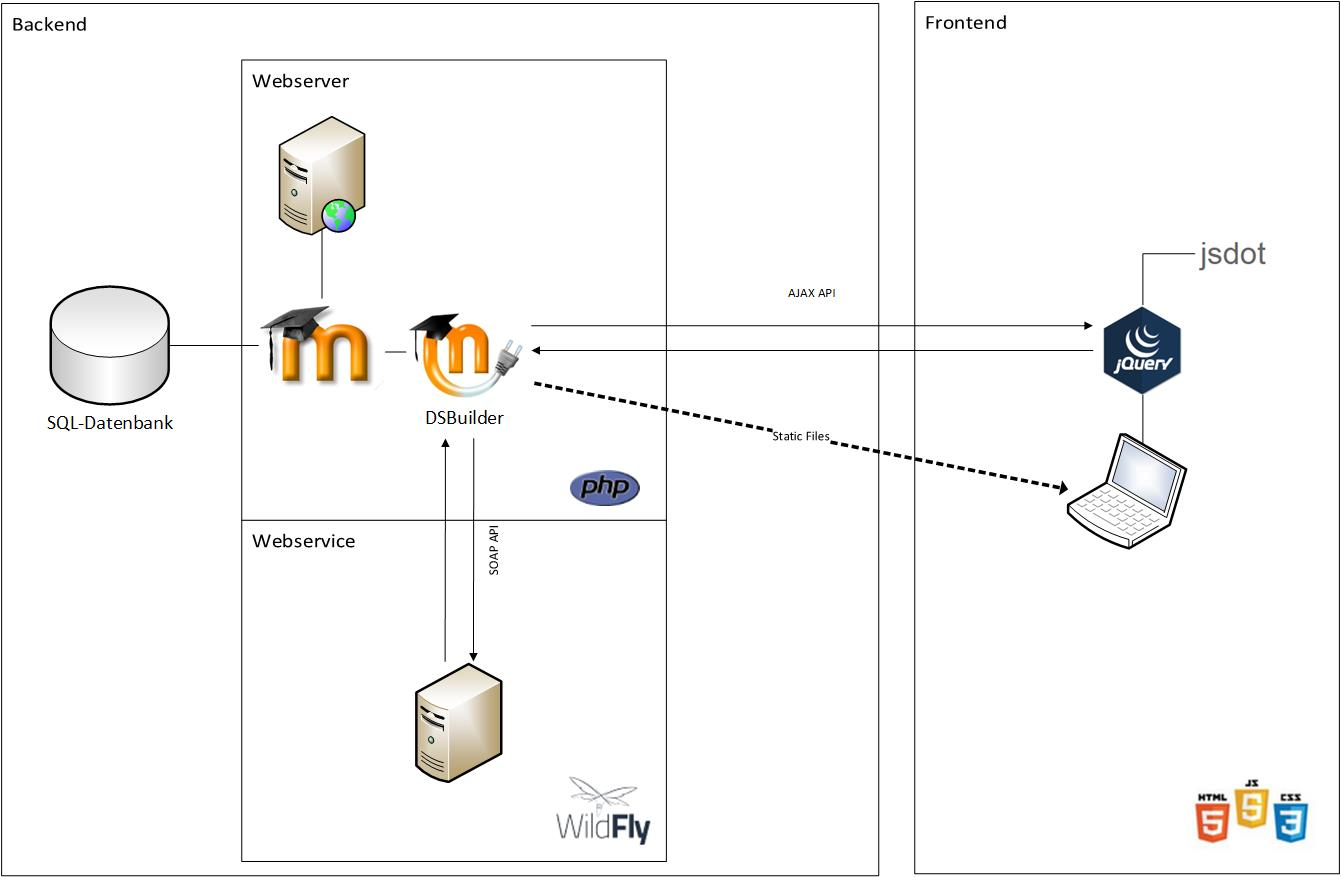
\includegraphics[width=0.9\textwidth]{graphics/UeberblickTechnologien.jpg}
  \caption{Technischer �berblick}
  \label{fig:technoloieUeberblick}
\end{figure}

Auf Clientseite wird HTML mit CSS und JavaScript verwendet, um das Modul f�r den Benutzer darstellen zu k�nnen. Als JavaScript-Frameworks wird jQuery und und als JavaSrcipt-Applikation wird jsdot eingesetzt. �ber jQuery ist die Kommunikation mit dem Moodlemodul �ber das AJAX-Protokoll organisiert. Jsdot dient als Grapheditor.  

\subsubsection{Datenstruktur-Verarbeitungsservice}  
\label{sec:technWebService}


Der Datenstruktur-Verarbeitungsservice hat die Aufgabe Datenstrukturen in Form eines JSON Strings f�r das Moodlemodul bereitzustellen. Hierf�r muss der Lehrende zuvor eine Wrapperdatei auf Basis eines vorgegebenen Interfaces (vergl. Anhang Codebeispiel \ref{code:wrapper}) in Java implementieren und der Anwendung zur Verf�gung stellen. Diese Wrapperklasse dient als Schnittstelle zwischen dem Webservice und der Implementierung der Datenstruktur. Die wichtigen Funktionen, die durch die Implementierung dieses Interfaces zur Verf�gung gestellt werden sollten sind das Hinzuf�gen und L�schen von Schl�sseln, sowie das Erzeugen eines serialisierten JSON Strings aus der Datenstruktur und das Deserialisieren eines JSON Strings in die Datenstruktur.  
 
Um funktionsf�hig zu sein, muss der Datenstruktur-Verarbeitungsservice den vom Lehrenden bereitgestellten Code kompilieren und ausf�hren. Der Verarbeitungsservice ist als separater Webservice implementiert und wird somit von einem anderen Server aus bereitgestellt. Die Separierung des Systems erfolgt aus den Risiken, dass der Code sch�dlich sein oder eine schlechte Ausf�hrungsleistung aufweisen kann. Durch die Trennung der beiden Systeme kann in beiden F�llen Zusammen- oder Performanceeinbr�chen der gesamten E-Learning-Plattform vorgebeugt werden. Weiterhin kann so Datendiebstahl verhindert werden, da in der Verarbeitungsumgebung keine nutzerbezogenen Daten verarbeitet werden. Bei Ausfall des Verarbeitungsservices ist jedoch das Aufrufen eines n�chsten Schrittes nicht mehr m�glich \cite{Usener2014}.

Der Webservice verf�gt �ber die SOAP-Schnittstellen  \textit{analyzeSourceCode}, \textit{assignmentInitialize} und \textit{assignmentIsIntialized}, die zur Initialisierung einer neuen DSBuilder-Instanz be�tigt werden, ebenso wie die SOAP-Schnittstellen \textit{submissionGetNextInput} und \textit{submissionGetInitialDS}, die zur Verarbeitung einer Datenstruktur ben�tigt werden. Um den Webservice nutzen zu k�nnen m�ssen ihm Codedateien zu Verf�gung gestellt werde. �ber den SOAP-Aufruf \textit{analyzeSourceCode} wird die Lesbarkeit der Dateien gepr�ft. Anschlie�end kann �ber den SOAP-Aufruf \textit{assignmentInitialize} der Code compiliert und bereitgestellt werden. Die Ausf�hrung des Codes ist vor jedem Einf�gen, das von einem Studierenden durchgef�hrt wird, notwendig.
So kann �ber den SOAP-Aufruf \textit{submissionGetNextInput} der der n�chste �bungsschritt f�r den Studierenden erhalten werde. Bei der Initialisierung der �bung wird der SOAP-Aufruf \textit{submissionGetInitialDS} ben�tigt. Die Antwort auf diese beiden Aufrufe beinhaltet den neuen Schl�ssel, die serialisierte Datenstruktur und zus�tzliche Hilfe. 


\subsubsection{Moodlemodul backendseitig}
\label{sec:dsbuilderbackend}
Das backendseitige Moodlemodul besitzt die grundlegende Struktur eines Moodlemoduls, wie sie in Kapitel \ref{sec:modularten} dargestellt wurde. Die weiteren, f�r die Funktionalit�t des Moduls wichtigen Dateien sind die Dateien \pfile{renderer.php} und \pfile{render}- \pfile{able.php}, welche den DOM-Code generieren, die Dateien \pfile{ajax\_request.php} und \pfile{ajax\_helper.php}, welche das Handling von AJAX-Anfragen �bernehmen und die Datei \pfile{lib/js\_dot\_convert.php}, welche die Funktionen zur Verarbeitung der Datenstrukturen zur Verf�gung stellt. Im weiteren Verlauf dieses Abschnittes werden diese drei Funktionalit�ten tiefgehender erl�utert und Codeausschnitte exemplarisch vorgestellt.

\paragraph{Generierung des DOM-Codes} \hfill \\
Die Datei, welche f�r die Generierung des DOM-Codes verantwortlich ist, ist die \pfile{renderer.php}. Die Datei \pfile{renderable.php} implemeniert hingegen ein Interface, welches f�r die Verwendung des moodleinternen Renderers notwendig ist \cite{moodleRenderer}. Die in der Datei  \pfile{renderer.php} enthaltende Klasse \pfile{mod\_dsbuilder\_renderer} enth�lt Funktionen zum Erstellen der f�r den DSBuilder ben�tigten Ansichten. So k�nnen �bersichten �ber laufende oder eingereichte Abgaben oder Notentabellen generiert werden.
\begin{figure}[htbp] 
\lstinputlisting[language=PHP, caption=Aufruf zur Initialisierung eines JSDot-Graphs, frame=single, label=code:initGraphEditor]{code/initDSBuilder.php}
\end{figure}
Ebenso k�nnen Ansichten zur Aufgabenbearbeitung generiert werden. Hierbei �bernimmt die Initiierung des Grapheneditors, welche im Quellcode \ref{code:initGraphEditor} dargestellt wird, eine zentrale Rolle. Es wird eine Hilfsfunktion des Moodle-API \cite{moodleJsApi} verwendet, welche die frontendseitige JavaScript-Funktion zur Initialisierung des Grapheneditors anst��t. Die frontendseitige Funktionalit�t wird im Kapitel \ref{sec:dsbuilderfrontend} vertieft.

\paragraph{Modulinterne AJAX-API} \hfill \\
Zur asynchronen Daten�bertragung zwischen Browser und Server stellt das Moodlemodul eine AJAX Api zur Verf�gung. 
\pfile{ajax\_helper.php} definiert.
\begin{figure}[htbp] 
\lstinputlisting[language=PHP, caption=Ausschnitt AJAX API, frame=single, label=code:ajax]{code/ajax.php}
\end{figure}
Der Quellcode \ref{code:ajax} zeigt einen Codeausschnitt aus der \pfile{ajax\_request.php}, in dem die m�glichen Aktionen definiert sind, die nach einer AJAX-Anfrage durchgef�hrt werden k�nnen. Hierbei handelt es sich um die Funktionen, welche �ber die Kn�pfe unterhalb des Grapheneditors (vergl. Kapitel \ref{sec:funktionalitaet}, Abschnitt \textit{Studierender}) angesto�en werden k�nnen. Explizit handelt es sich um die Funktionen \textit{Syntax pr�fen} (Quellcode \ref{code:ajax}, Z. 2), \textit{Speichern und weiter} (Quellcode \ref{code:ajax}, Z. 6) und \textit{Letzten Schritt wiederholen} (Quellcode \ref{code:ajax}, Z. 10). Die jeweils angesto�enen Funktionen sind in der 
Von dort aus werden weitere Funktionen zur Datenstrukturverarbeitung in der Klasse \pfile{jsdot\_graph} angesto�en. Diese Funktionen werden im n�chsten Abschnitt vertiefender behandelt.

\paragraph{Die Datenhaltung} \hfill \\
Das Modul DSBuilders ben�tigt vier Entit�ten f�r seine Datenhaltung. Es handelt sich um die Entit�ten \textit{DSBuilder}, \textit{Assigment File}, \textit{Submission} und \textit{Submission Step}. Die Abbildung \ref{fig:erm} zeigt das Datenmodell des Moduls. 
\begin{figure}[htbp] 
  \centering
     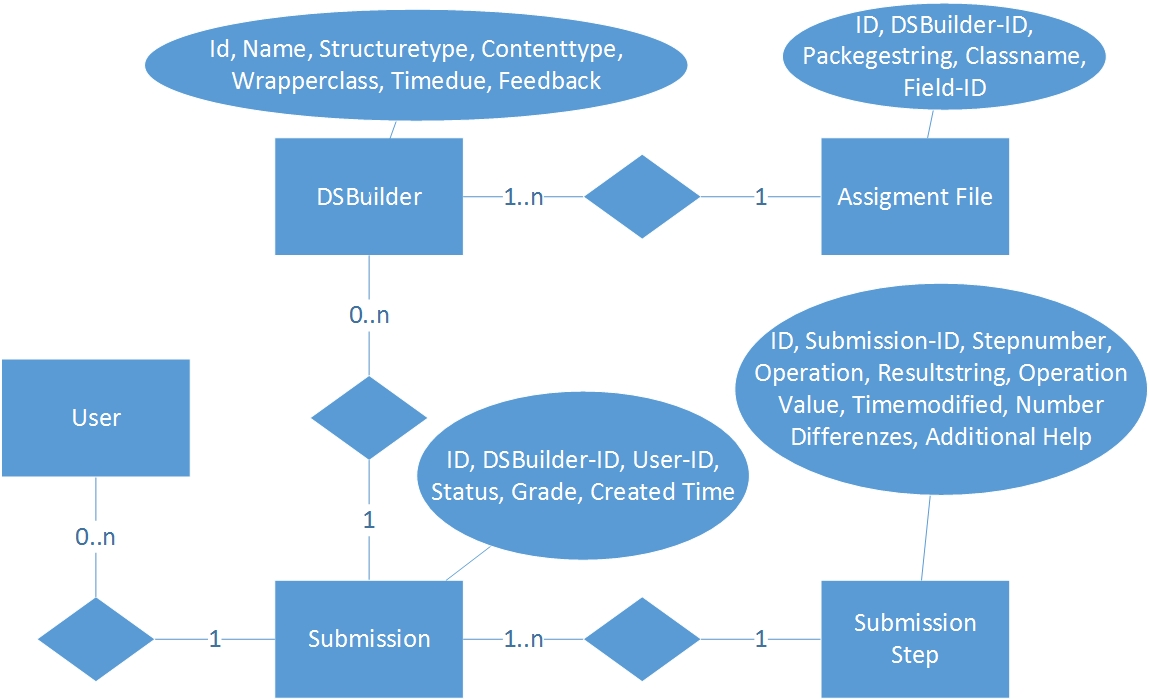
\includegraphics[width=0.9\textwidth]{graphics/ERM.jpg}
  \caption{Datenmodell des DSBuilders}
  \label{fig:erm}
\end{figure}
Nachdem das Modul neu in einem Kurs initialisiert worden ist, wird ein neues Datum der Entit�t \textit{DSBuilder} angelegt. Die der neuen Instanz des Moduls vom Lehrenden zugewiesenen Javadateien werden als Datum der Entit�t \textit{Assigment File}  gespeichert. Sobald Studierende die Instanz nutzen, wird f�r jeden Studierenden mit Vermerk auf die Instanz ein neues Datum der Entit�t \textit{Submission} angelegt. Jeder \textit{Submission} werden \textit{Submission Steps} zugeordnet. Sie beinhalten Informationen �ber die jeweiligen ausgef�hrten Schritte. 

\paragraph{Die Datenstrukturverarbeitung} \hfill \\
In der Datei \pfile{lib/js\_dot\_convert.php} liegt die Funktionalit�t der Datenstrukturverarbeitung. In ihr sind vier Klassen implementiert, von denen die Klasse \pfile{jsdot\_ graph} eine Schnittstelle zur Konvertierung einer Datenstruktur zwischen dem Grapheneditor im Frontend und der Datenhaltung im Backend bietet. Des weiteren repr�sentiert diese Klasse die Datenstruktur, die im jsdot-Editor zur Pr�sentation eines Baumes gebraucht wird. Da ein jsdot-Graph �ber Knoten und Kanten verf�gt, werden diese Elemente in der Datei \pfile{lib/js\_dot\_convert.php} durch die Klassen \pfile{jsdot\_edge} und \pfile{jsdot\_node} repr�sentiert. Spezifischere Erl�uterungen zu den jsdot-Elemente sind in Kapitel \ref{sec:dsbuilderfrontend} zu finden.
Abbildung \ref{fig:umlJsDotConvert} zeigt ein UML-Klassendiagramm der vier Klassen.
\begin{figure}[htbp] 
  \centering
     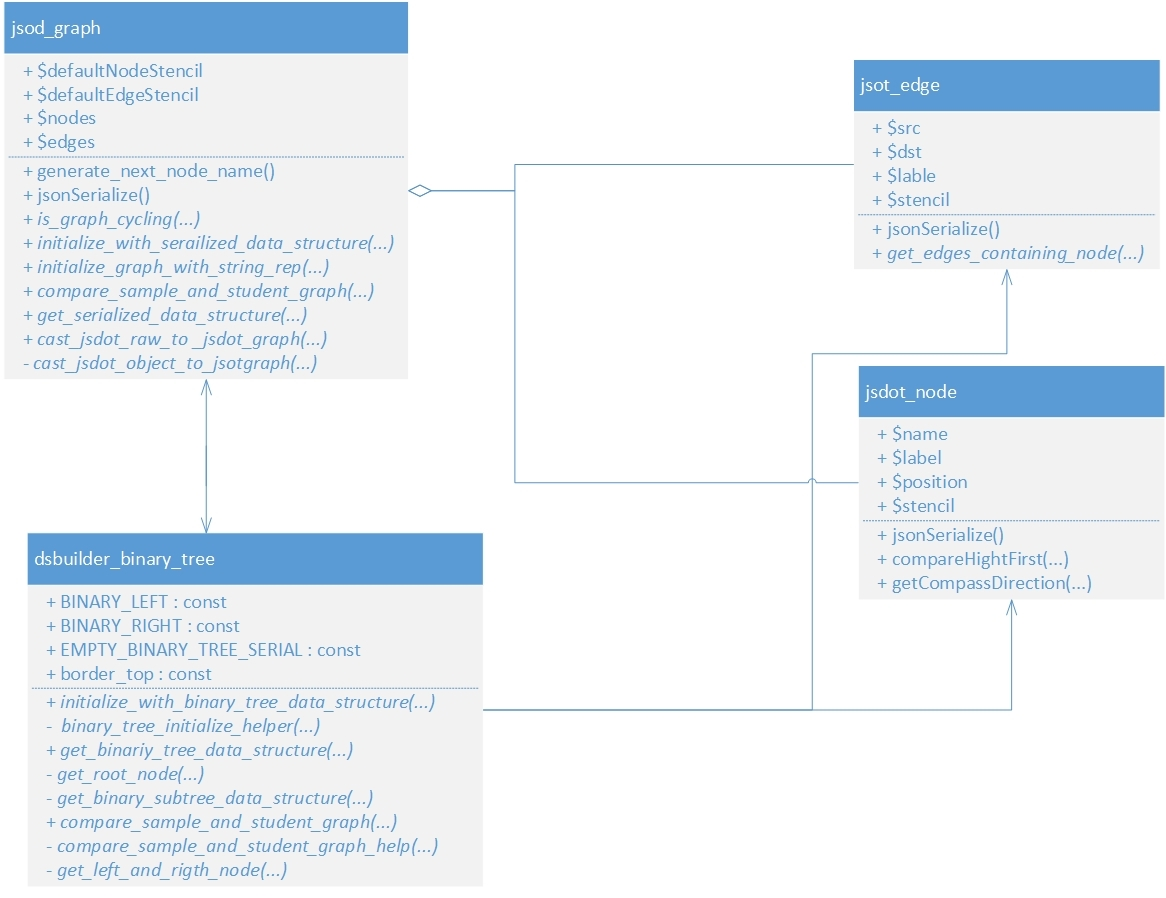
\includegraphics[width=0.9\textwidth]{graphics/UMjsDotConvert1.jpg}
  \caption{UML js\_dot\_convert}
  \label{fig:umlJsDotConvert}
\end{figure}
Die Funktionalit�t zur Umwandlung zwischen Datenstrukturen f�r den jsdot-Editor und den Webservice stellt die Klasse \pfile{dsbuilder\_binary\_tree} bereit. 

Die drei �ffentlichen Funktionen der Klasse \pfile{dsbuilder\_binary\_tree}, die die wichtigen Funktionalit�ten zur Verarbeitung der Datenstruktur bereitstellen, sind die statischen Funktionen 
\textit{initialize\_with\_binary\_tree\_data\_structure(...)}, \textit{get\_bi- nary\_tree\_data\_ structure(...)} und \textit{compare\_sample\_and\_student\_graph(...)}. Hierbei erm�glichen die erste Funktionen die Umwandlung der Datenstruktur, die der Webservice liefert, in die Datenstruktur f�r den jsdot-Editor. Die zweite Funktion erm�glicht die Umwandlung in die umgekehrte Richtung. Die dritte Funktion vergleicht zwei Graphen und markiert die sich unterscheidenden Knoten. Sie wird f�r die Feedbackfunktion genutzt. Im folgenden werden die Funktionen tiefgehender vorgestellt.

\subsubsection{Moodlemodul frontendseitig}
\label{sec:dsbuilderfrontend}
Die im Vordergrund stehende Funktionalit�t des Fronends ist die von der JavaScript-Applikation jsdot bereitgestellte Grapheneditor. In diesem Grapheneditor  werden von Elemente zur Verf�gung gestellt, die vom Studierenden bearbeitet werden k�nnen. 
Die Funktionalit�t zur Verarbeitung der Nutzereingaben wird �ber die Datei \pfile{dsbuilder.js} bereitgestellt.
Des weiteren stellt diese Datei die AJAX-Kommunikation zur Verf�gung.

\paragraph{Der Grapheneditor} \hfill \\
Der Grapheneditor wird durch die JavaScript-Applikation jsdot bereitgestellt. So kann jsdot �ber das HTML-Element \textit{svg} Knoten und Kanten bereitstellen, die editierbar sind. Aus diesen Elementen k�nnen Strukturen wie Graphen, B�ume oder Listen erstellt werden. Der Codeauszug \ref{code:initJsDot} zeigt die Initialisierung eines neuen jsdot-Graphen. 
\begin{figure}[htbp] 
\lstinputlisting[language=JavaScript, caption=Initiierung eines JsDot-Graphs, frame=single, label=code:initJsDot]{code/initJsDot.js}
\end{figure}
Weiterhin stellt jsdot eine API zur Verf�gung. �ber diese API k�nnen  neue Elemente zu einem Graphen hinzugef�gt werden. Ebenso k�nnen bestehende Elemente ge�ndert oder ausgelesen werden. Au�erdem kann bei der Initialisierung eines Graphen eingestellt werden, ob der Graph im Bearbeitungsmodus oder im Anzeigemodus bereitgestellt wird. Codebeispiel \ref{code:initJsDot} zeigt die Initialisierung eines Graphen im Bearbeitungsmodus. 
So wird der Editiermodus verwendet, um einen editierbaren Graphen f�r die Aufgabenbearbeitung zur Verf�gung zu stellen (vergl. Kapitel \ref{sec:funktionalitaet} Abb. \ref{fig:editor} oben). Der Anzeigemodus wird hingegen f�r das Feedback verwendet (vergl. Kapitel \ref{sec:funktionalitaet} Abb. \ref{fig:editor} unten). Im Frontend findet keine Verarbeitung der Graphen-Datenstruktur statt. Die Graphen-Datenstruktur wird �ber die im folgenden Abschnitt erl�uterte AJAX-API an das Backend gesendet und dort verarbeitet (vergl. Kapitel \ref{sec:dsbuilderbackend} Abschnitt \textit{Datenstrukturverarbeitung}).

\paragraph{AJAX-Api des Frontends} \hfill \\
Das Frontend stellt eine AJAX-API zur Echtzeitkommunikation mit dem Moodlemodul bereit. �ber die Kn�pfe unterhalb des Grapheneditors (vergl. Kapitel \ref{sec:funktionalitaet}, Abschnitt \textit{Studierender}) k�nnen die Funktionen der API angesto�en werden. Die Verarbeitung der AJAX-Anfragen wurde bereits in Kapitel \ref{sec:dsbuilderbackend} im Abschnitt \textit{Modulinterne AJAX-API} erl�utert. �ber AJAX-Anfragen werden Informationen wie die Graphen-Datenstruktur, das Feedback und m�gliche Fehler �bertragen.


 \bibliography{Bachelorarbeit}
  \bibliographystyle{alpha}
 

  \diplomabschlusserklaerung{(Abgabedatum)}
\end{document}
